\section{Results}\label{section:results}
After implementing the algorithms described in \autoref{section:algorithms-used}, experimental results were retrieved.
These results range from number of operation, elapsed time and relative error.
The results were taken in a machine with the AMD Ryzen 5 5600X processor and implemented in Python 3.

For the exhaustive search algorithm, the results obtained are presented in \autoref{tab:ex-table}, \autoref{fig:ex-op}, and \autoref{fig:ex-time}.
In \autoref{tab:ex-table}, $V$ and $E$ are the number of vertices and edges of the graph; $p$ is the fraction between $E$ and the maximum number of edges; execution time is the time elapsed during the computation of the algorithm;
number of basic operations is how many basic operations (defined in \autoref{section:formal-analysis}) took place; number of dominating sets is the number of sets generated that were dominating sets; and the time per operation is the estimated elapsed time for a basic operation.
From this data we can verify that the number of basic operations presents an exponential order of growth ($1^{0.693x}=2^x$, $R^2=1$, \autoref{fig:ex-op}), following the behavior expected by \autoref{eq:ex-closed-formula} and \autoref{eq:ex-big-o}.
The execution time also presents an exponential growth ($2.74e\scalebox{0.5}[1.0]{\( - \)}5^{0.712x}$, $R^2=1$, \autoref{fig:ex-time}) with the number of edges.
The time per basic operation in seconds is $3,71e\scalebox{0.5}[1.0]{\( - \)}5 \pm 8,36e{\scalebox{0.5}[1.0]{\( - \)}6}$.
From these experiences, the largest graph able to be computed was one with 9 vertices and 23 edges (\autoref{fig:9-05-ex}).
\autoref{eq:ex-time-calc} is used to calculate how long a computation takes using the same hardware.


\begin{table}[ht!]
\caption{Results from exhaustive search algorithm}
\label{tab:ex-table}
\resizebox{0.5\textwidth}{!}{%
\begin{tabular}{ccccccc}
\multirow{3}{*}{V} & \multirow{3}{*}{p} & \multirow{3}{*}{E} & \multirow{3}{*}{\begin{tabular}{c} Execution \\ Time (s) \end{tabular}} & \multirow{3}{*}{\begin{tabular}{c} \# of \\ Basic \\Operations\end{tabular}} & \multirow{3}{*}{\begin{tabular}{c} \# of \\ Dominating \\Sets\end{tabular}} & \multirow{3}{*}{\begin{tabular}{c}Time per \\ Operation (s)\end{tabular}} \\ 
& & & & & & \\
& & & & & & \\
\hline
4 & 0,125 & 4 & 7,89E-04 & 16 & 13 & 5,26E-05 \\
4 & 0,25 & 6 & 2,68E-03 & 64 & 57 & 4,26E-05 \\
4 & 0,5 & 6 & 2,57E-03 & 64 & 57 & 4,07E-05 \\
4 & 0,75 & 6 & 2,76E-03 & 64 & 57 & 4,38E-05 \\
5 & 0,125 & 4 & 6,00E-04 & 16 & 11 & 4,00E-05 \\
5 & 0,25 & 6 & 3,22E-03 & 64 & 49 & 5,11E-05 \\
5 & 0,5 & 7 & 5,12E-03 & 128 & 107 & 4,03E-05 \\
5 & 0,75 & 8 & 1,06E-02 & 256 & 227 & 4,15E-05 \\
6 & 0,125 & 5 & 1,22E-03 & 32 & 21 & 3,93E-05 \\
6 & 0,25 & 8 & 6,64E-03 & 256 & 203 & 2,61E-05 \\
6 & 0,5 & 12 & 1,74E-01 & 4096 & 3835 & 4,24E-05 \\
6 & 0,75 & 13 & 2,33E-01 & 8192 & 7823 & 2,85E-05 \\
7 & 0,125 & 6 & 1,59E-03 & 64 & 33 & 2,53E-05 \\
7 & 0,25 & 10 & 2,76E-02 & 1024 & 871 & 2,70E-05 \\
7 & 0,5 & 15 & 1,21E+00 & 32768 & 31017 & 3,71E-05 \\
7 & 0,75 & 18 & 1,14E+01 & 262144 & 256281 & 4,34E-05 \\
8 & 0,125 & 8 & 6,32E-03 & 256 & 159 & 2,48E-05 \\
8 & 0,25 & 12 & 1,15E-01 & 4096 & 3407 & 2,80E-05 \\
8 & 0,5 & 18 & 9,86E+00 & 262144 & 247957 & 3,76E-05 \\
8 & 0,75 & 23 & 3,51E+02 & 8388608 & 8274471 & 4,19E-05 \\
9 & 0,125 & 10 & 2,63E-02 & 1024 & 731 & 2,57E-05 \\
9 & 0,25 & 17 & 4,03E+00 & 131072 & 118053 & 3,07E-05 \\
9 & 0,5 & 23 & 3,61E+02 & 8388608 & 8064383 & 4,30E-05
\end{tabular}%
}
\end{table}

\newpage

\begin{figure}[!ht]
    \centering
    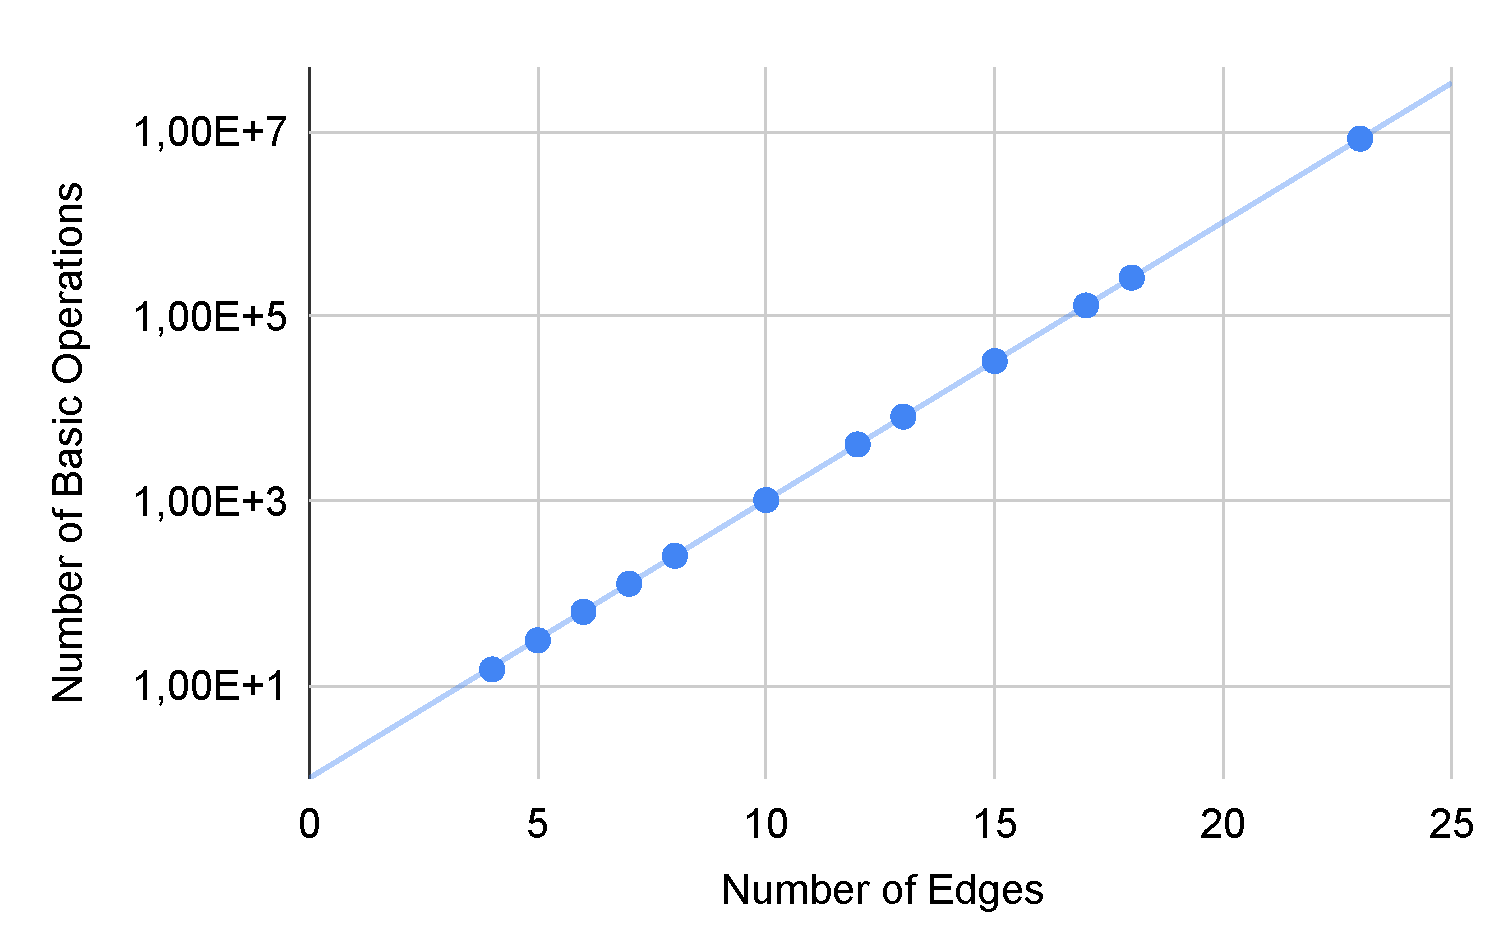
\includegraphics[width=0.9\linewidth]{figs/ex-basic-operations.pdf}
    \caption{Correlation between number of edges and number of basic operation for exhaustive search. Logarithmic scale.}
    \label{fig:ex-op}
\end{figure}

\begin{figure}[!ht]
    \centering
    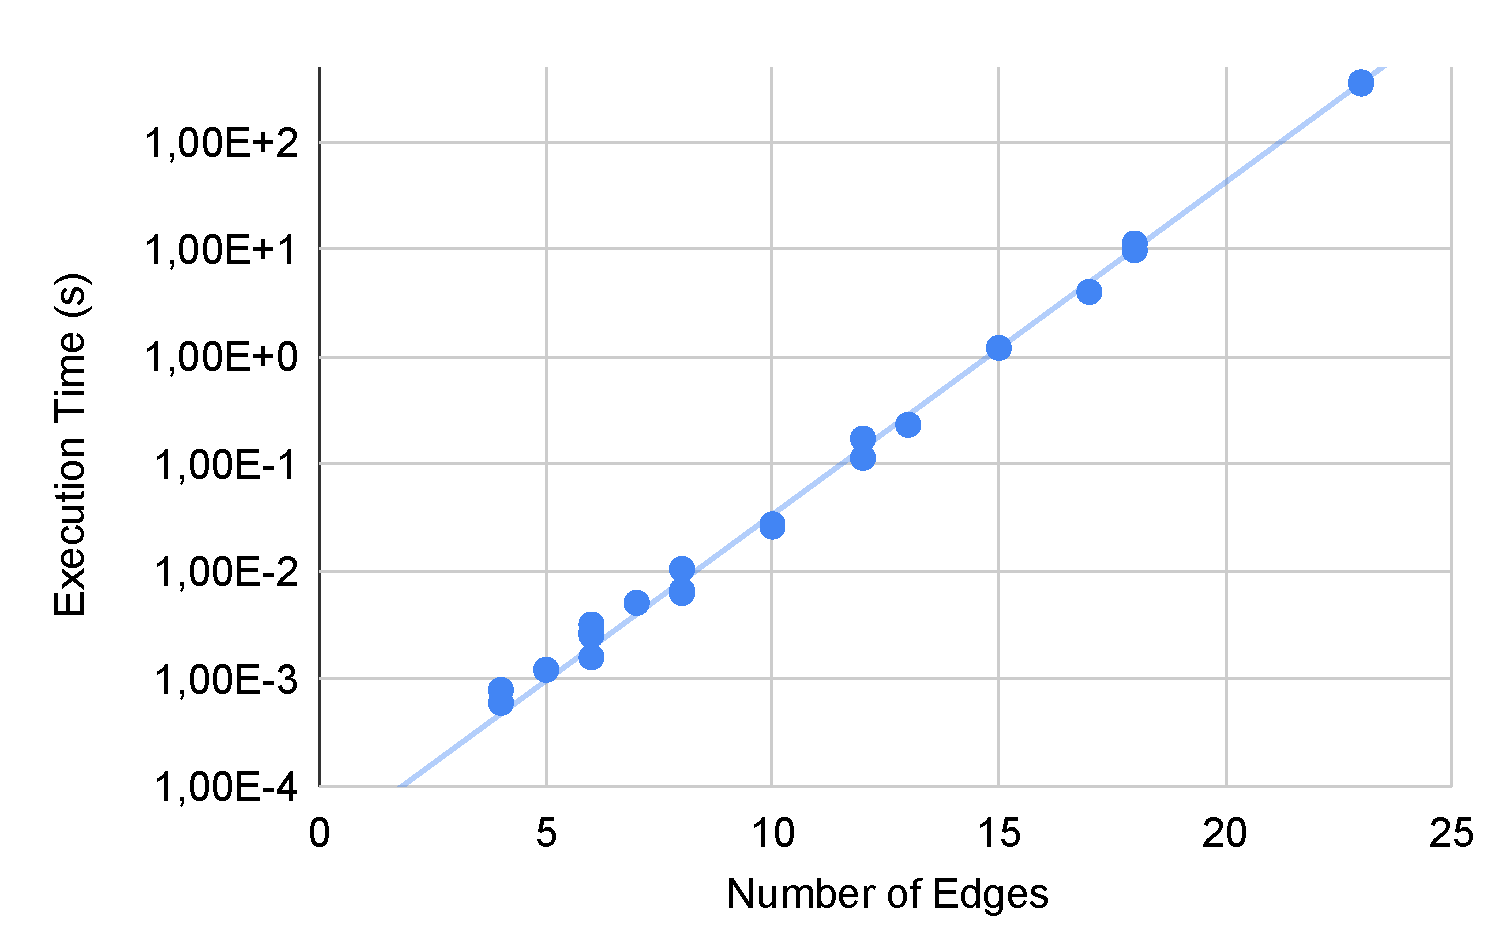
\includegraphics[width=0.9\linewidth]{figs/ex-time.pdf}
    \caption{Correlation between number of edges and elapsed time for exhaustive search. Logarithmic scale.}
    \label{fig:ex-time}
\end{figure}

\begin{figure}[!ht]
    \centering
    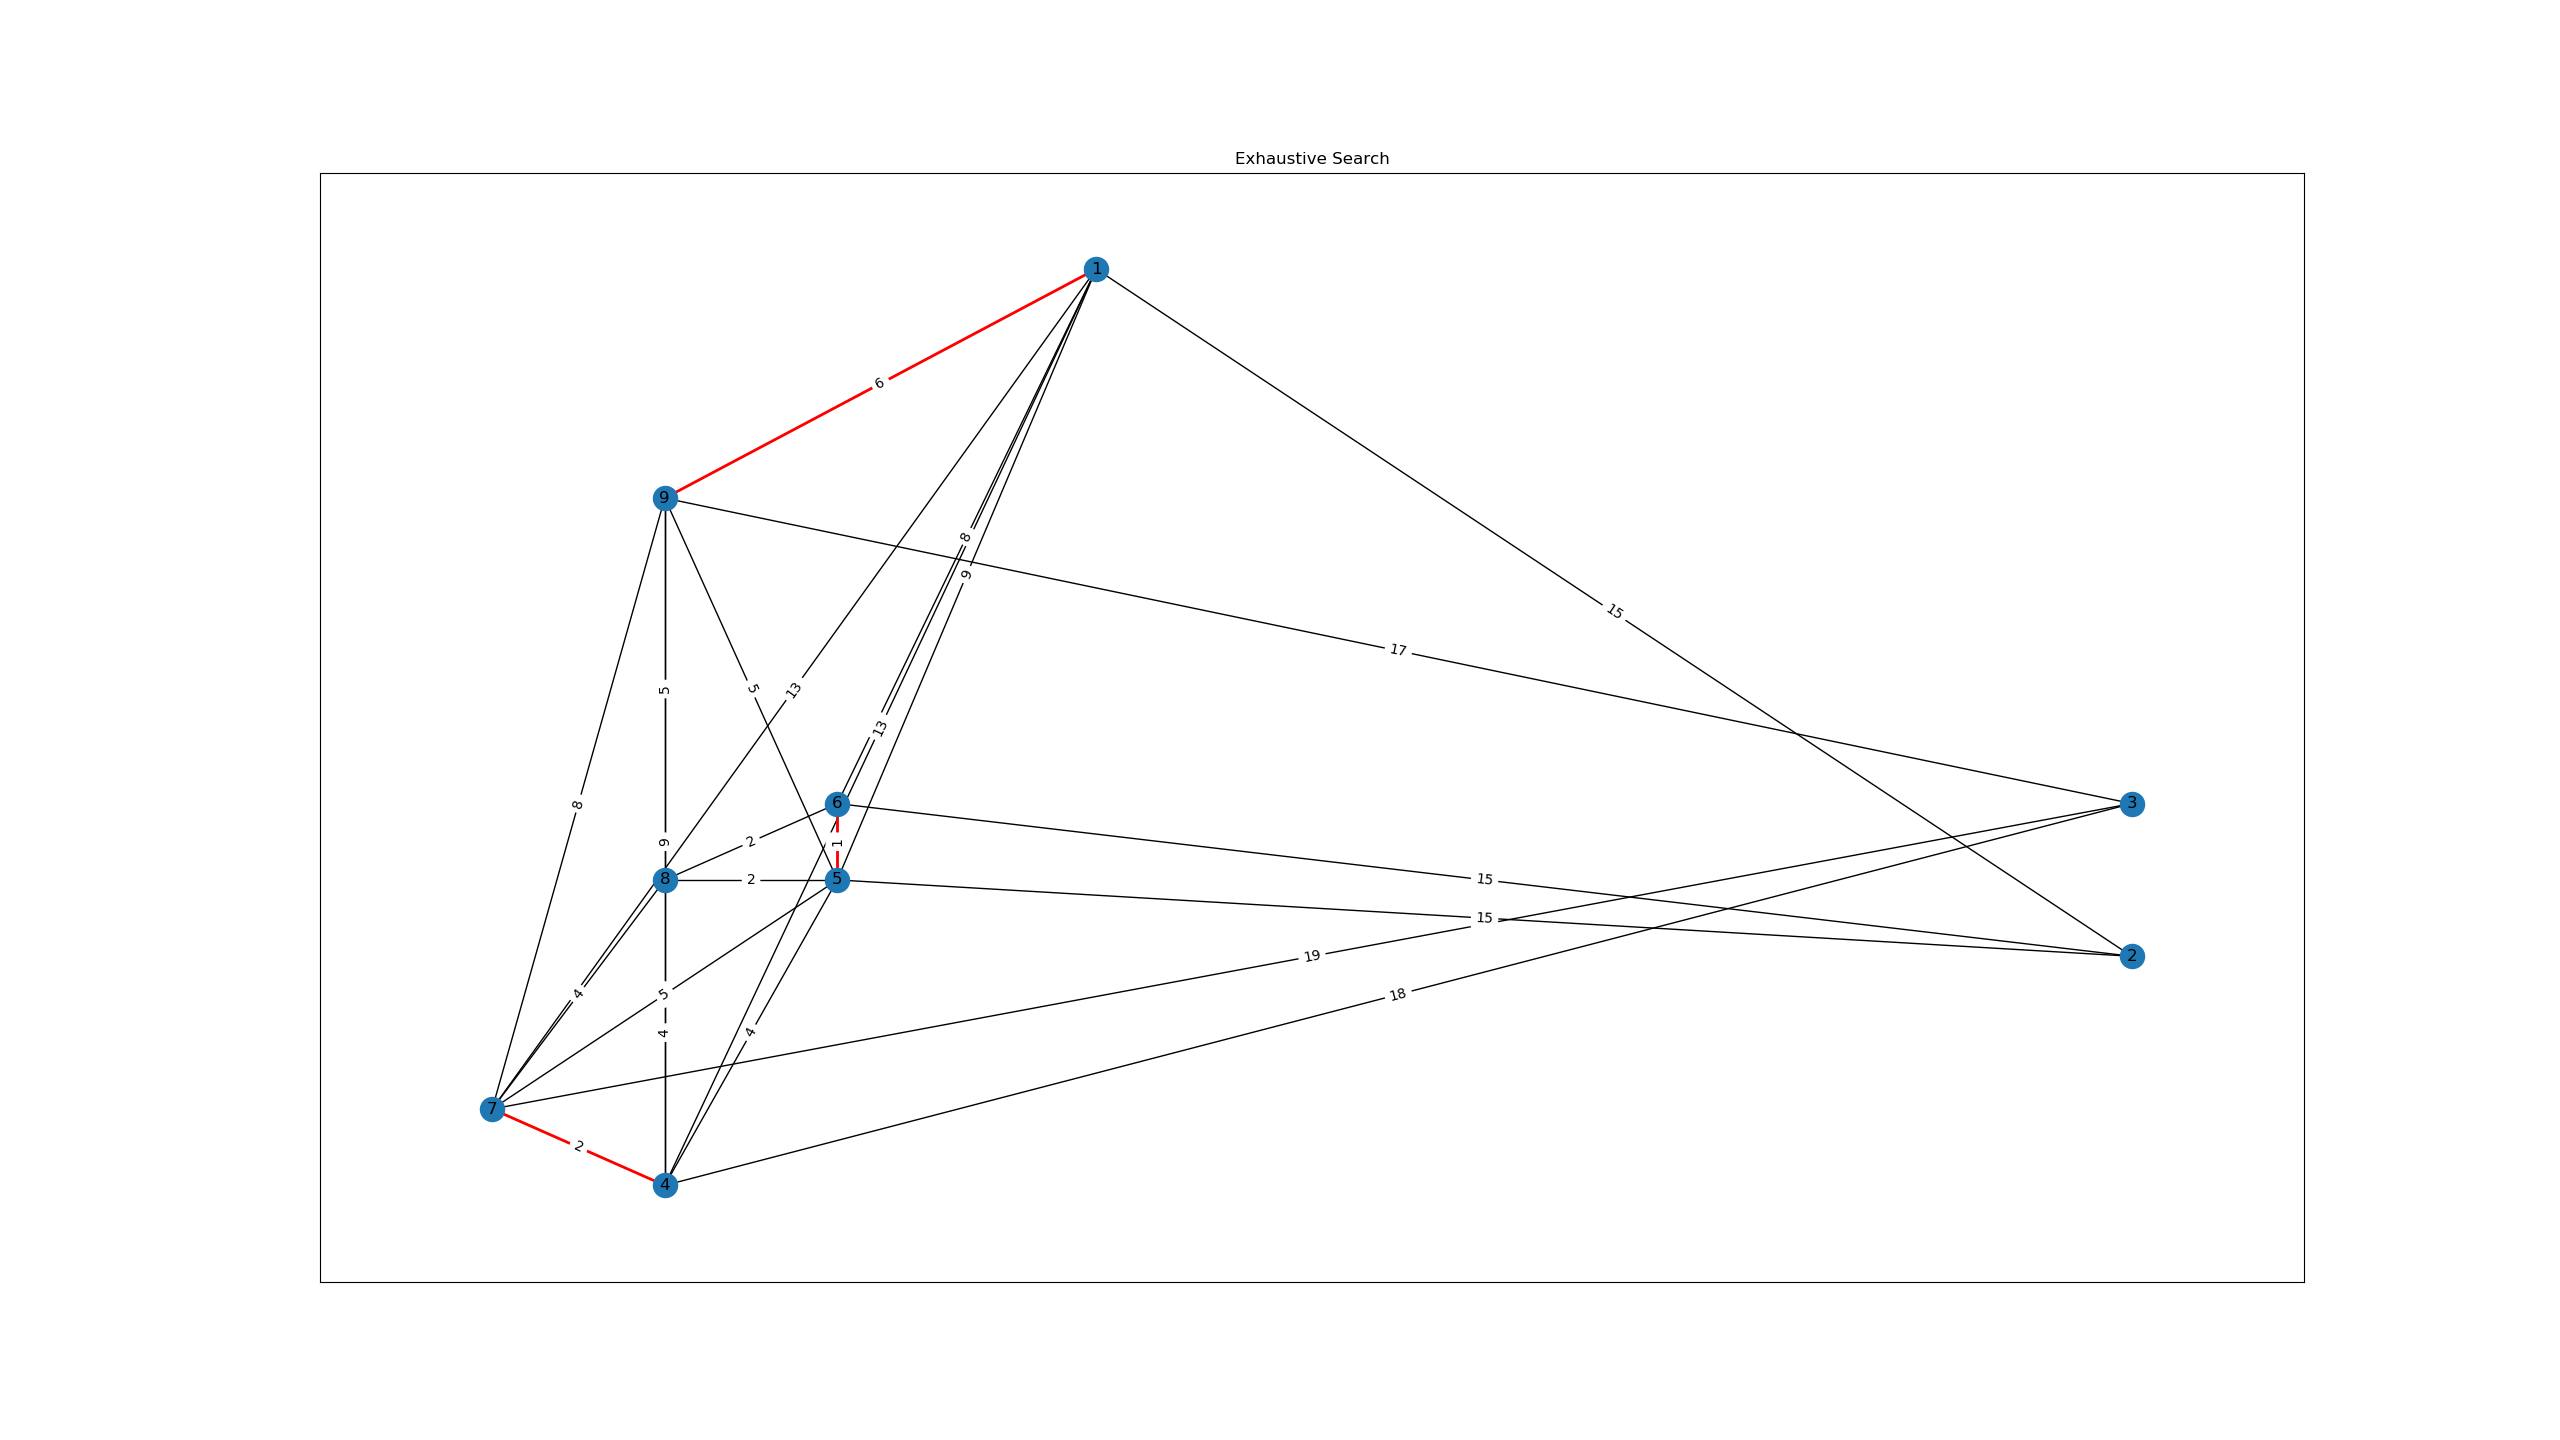
\includegraphics[width=1\linewidth]{figs/fig-9-0.5-exhaustive}
    \caption{Largest graph able to be processed. 9 nodes and 23 edges.}
    \label{fig:9-05-ex}
\end{figure}

\begin{equation}
    time = T(n) * 3,71e\scalebox{0.5}[1.0]{\( - \)}5 = 2^n * 3,71e\scalebox{0.5}[1.0]{\( - \)}5
    \label{eq:ex-time-calc}
\end{equation}

\newpage

For the minimum weight greedy heuristics, the results obtained are presented in \autoref{tab:minw-table}, \autoref{fig:minw-sol}, \autoref{fig:minw-time}, and \autoref{fig:minw-ratio}. 
The columns for \autoref{tab:minw-table} are equal to the ones in \autoref{tab:ex-table}, with the exception of: number of solutions tested, which is the number of sets tested before a dominating one was formed; and accuracy ratio, which is a measure used to compare the weight of the solution obtained with the weight of the optimal solution. 
This data verifies that the number of solutions tested grows with the number of edges.
The elapsed time increases with the number of edges.
From the accuracy ratio, it can be inferred that the algorithm is relatively accurate in smaller graph, becoming less accurate in larger graphs.


\begin{table}[ht!]
\caption{Results from minimum weight greedy algorithm}
\label{tab:minw-table}
\resizebox{0.5\textwidth}{!}{%
\begin{tabular}{ccccccc}
\multirow{3}{*}{V} & \multirow{3}{*}{p} & \multirow{3}{*}{E} & \multirow{3}{*}{\begin{tabular}{c} Execution \\ Time (s) \end{tabular}} & \multirow{3}{*}{\begin{tabular}{c}\# of\\ Solutions\\Tested\end{tabular}} & \multirow{3}{*}{\begin{tabular}{c} Accuracy \\ Ratio \end{tabular}}\\ 
& & & & & & \\
& & & & & & \\
\hline
4 & 0.125 & 4 & 1,05E-04 & 2 & 1,80 \\
4 & 0.25 & 6 & 1,03E-04 & 2 & 1,00 \\
4 & 0.5 & 6 & 9,78E-05 & 2 & 1,00 \\
4 & 0.75 & 6 & 1,15E-04 & 2 & 1,00 \\
5 & 0.125 & 4 & 7,20E-05 & 1 & 1,00 \\
5 & 0.25 & 6 & 1,05E-04 & 2 & 1,00 \\
5 & 0.5 & 7 & 9,78E-05 & 2 & 1,00 \\
5 & 0.75 & 8 & 1,08E-04 & 2 & 1,00 \\
6 & 0.125 & 5 & 9,58E-05 & 3 & 1,50 \\
6 & 0.25 & 8 & 1,03E-04 & 4 & 1,61 \\
6 & 0.5 & 12 & 1,05E-04 & 3 & 1,00 \\
6 & 0.75 & 13 & 9,87E-05 & 3 & 1,00 \\
7 & 0.125 & 6 & 8,51E-05 & 3 & 1,00 \\
7 & 0.25 & 10 & 1,11E-04 & 4 & 1,60 \\
7 & 0.5 & 15 & 1,78E-04 & 4 & 1,56 \\
7 & 0.75 & 18 & 2,03E-04 & 4 & 1,27 \\
8 & 0.125 & 8 & 8,85E-05 & 3 & 1,00 \\
8 & 0.25 & 12 & 8,03E-05 & 2 & 1,00 \\
8 & 0.5 & 18 & 1,34E-04 & 4 & 1,31 \\
8 & 0.75 & 23 & 3,10E-04 & 6 & 1,75 \\
9 & 0.125 & 10 & 1,48E-04 & 6 & 2,13 \\
9 & 0.25 & 17 & 1,96E-04 & 7 & 2,56 \\
9 & 0.5 & 23 & 5,75E-04 & 11 & 4,44
\end{tabular}%
}
\end{table}

\begin{figure}[!ht]
    \centering
    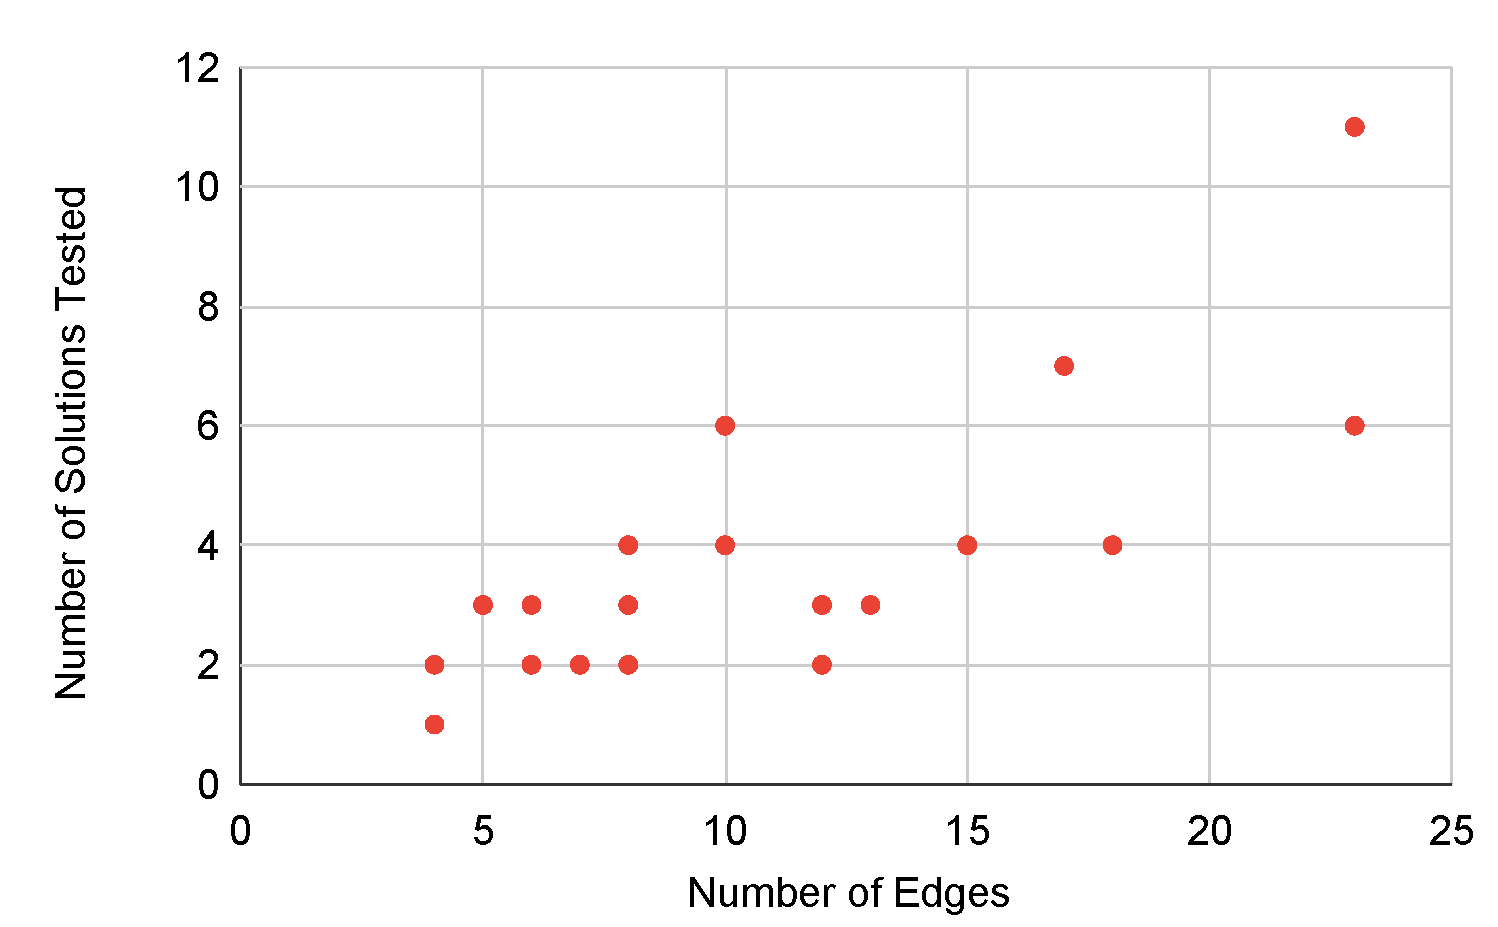
\includegraphics[width=0.9\linewidth]{figs/minw-solutions.pdf}
    \caption{Correlation between number of edges and number of solutions tested for minimum weight greedy algorithm.}
    \label{fig:minw-sol}
\end{figure}


\begin{figure}[!ht]
    \centering
    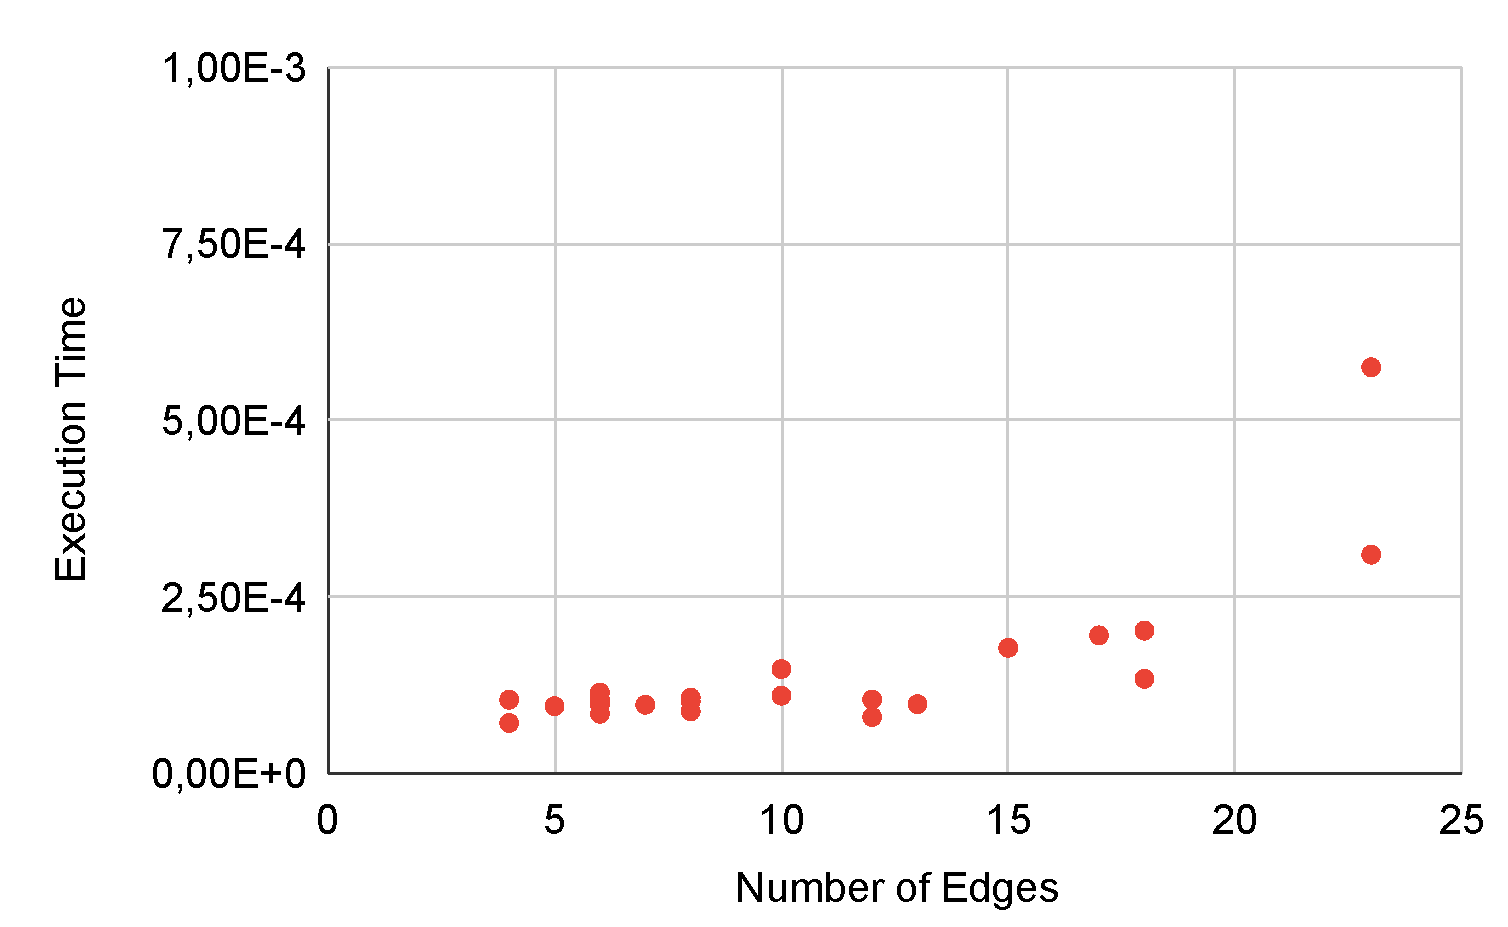
\includegraphics[width=0.9\linewidth]{figs/minw-time.pdf}
    \caption{Correlation between number of edges and elapsed time for minimum weight greedy algorithm.}
    \label{fig:minw-time}
\end{figure}

\newpage

\begin{figure}[!ht]
    \centering
    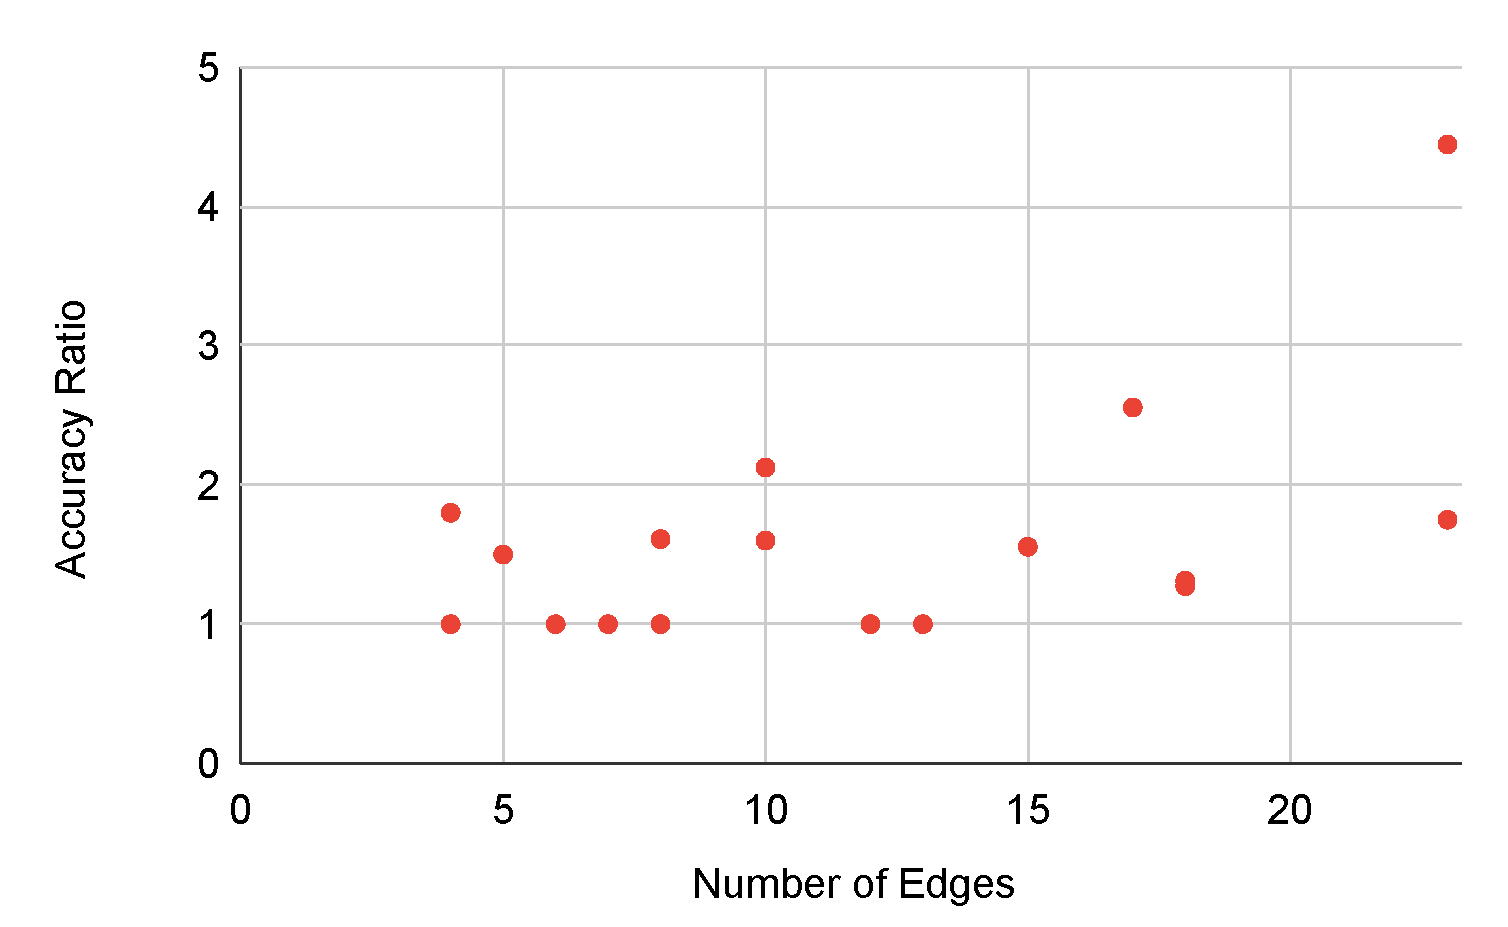
\includegraphics[width=0.9\linewidth]{figs/minw-ratio.pdf}
    \caption{Correlation between number of edges and accuracy ratio for minimum weight greedy algorithm.}
    \label{fig:minw-ratio}
\end{figure}


For the maximum connection greedy heuristics, the results obtained are presented in \autoref{tab:maxc-table}, \autoref{fig:maxc-sol}, \autoref{fig:maxc-time}, and \autoref{fig:maxc-ratio}. 
The columns for \autoref{tab:maxc-table} are equal to the ones in \autoref{tab:minw-table}.
The data shows that the number of solutions tested grows with the number of edges.
However, this growth is smaller than the previous heuristics.
The elapsed time increases with the number of edges, very similarly to the previous heuristics.
With the accuracy ratio, it can be stated that the algorithm, although not completely inaccurate, is not particularly accurate in smaller graphs.
However, the inaccuracy does not seem to grow, at least not in a noticeable rate, for larger graphs.


\begin{table}[ht!]
\caption{Results from maximum connection greedy algorithm}
\label{tab:maxc-table}
\resizebox{0.5\textwidth}{!}{%
\begin{tabular}{ccccccc}
\multirow{3}{*}{V} & \multirow{3}{*}{p} & \multirow{3}{*}{E} & \multirow{3}{*}{\begin{tabular}{c} Execution \\ Time (s) \end{tabular}} & \multirow{3}{*}{\begin{tabular}{c}\# of\\ Solutions\\Tested\end{tabular}} & \multirow{3}{*}{\begin{tabular}{c} Accuracy \\ Ratio \end{tabular}}\\ 
& & & & & & \\
& & & & & & \\
\hline
4 & 0.125 & 4 & 1,54E-04 & 1 & 1,00 \\
4 & 0.25 & 6 & 2,10E-04 & 2 & 1,13 \\
4 & 0.5 & 6 & 2,15E-04 & 2 & 1,13 \\
4 & 0.75 & 6 & 2,14E-04 & 2 & 1,13 \\
5 & 0.125 & 4 & 1,48E-04 & 1 & 1,00 \\
5 & 0.25 & 6 & 2,12E-04 & 2 & 2,00 \\
5 & 0.5 & 7 & 2,13E-04 & 2 & 1,00 \\
5 & 0.75 & 8 & 2,28E-04 & 2 & 1,08 \\
6 & 0.125 & 5 & 1,73E-04 & 2 & 1,69 \\
6 & 0.25 & 8 & 1,80E-04 & 3 & 1,89 \\
6 & 0.5 & 12 & 2,17E-04 & 3 & 1,36 \\
6 & 0.75 & 13 & 2,31E-04 & 3 & 2,14 \\
7 & 0.125 & 6 & 1,69E-04 & 3 & 1,58 \\
7 & 0.25 & 10 & 2,03E-04 & 2 & 1,80 \\
7 & 0.5 & 15 & 3,58E-04 & 3 & 2,11 \\
7 & 0.75 & 18 & 2,93E-04 & 3 & 1,27 \\
8 & 0.125 & 8 & 1,61E-04 & 2 & 1,35 \\
8 & 0.25 & 12 & 2,19E-04 & 3 & 3,27 \\
8 & 0.5 & 18 & 2,86E-04 & 4 & 2,06 \\
8 & 0.75 & 23 & 4,77E-04 & 3 & 1,19 \\
9 & 0.125 & 10 & 2,01E-04 & 3 & 1,63 \\
9 & 0.25 & 17 & 2,55E-04 & 3 & 1,44 \\
9 & 0.5 & 23 & 6,18E-04 & 4 & 3,22
\end{tabular}%
}
\end{table}

\begin{figure}[!ht]
    \centering
    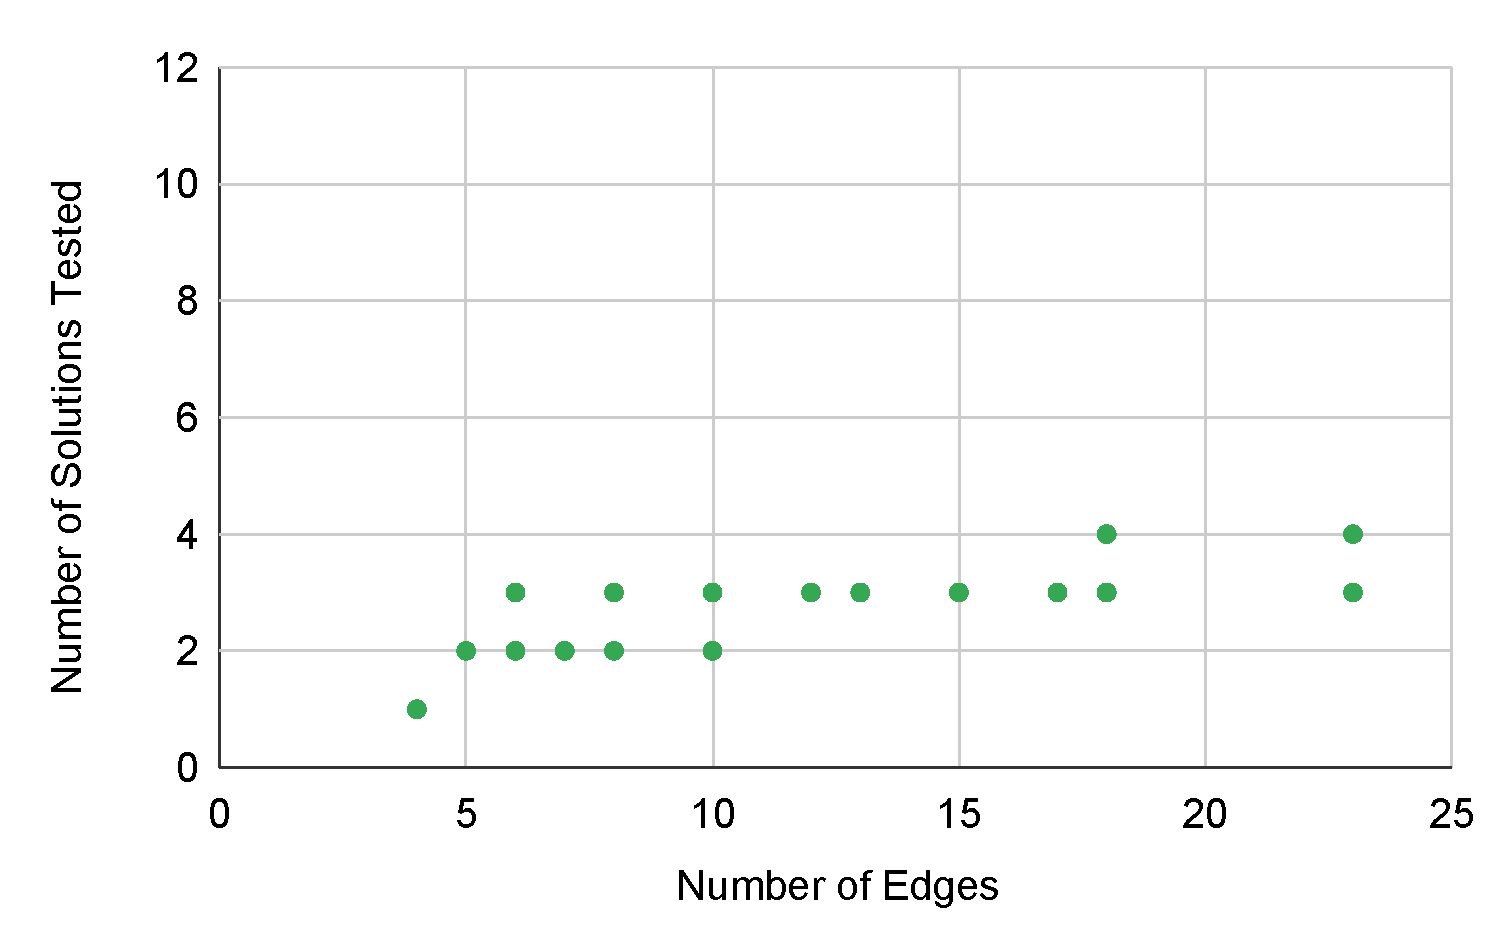
\includegraphics[width=0.9\linewidth]{figs/maxc-solutions.pdf}
    \caption{Correlation between number of edges and number of solutions tested for maximum connection greedy algorithm.}
    \label{fig:maxc-sol}
\end{figure}


\begin{figure}[!ht]
    \centering
    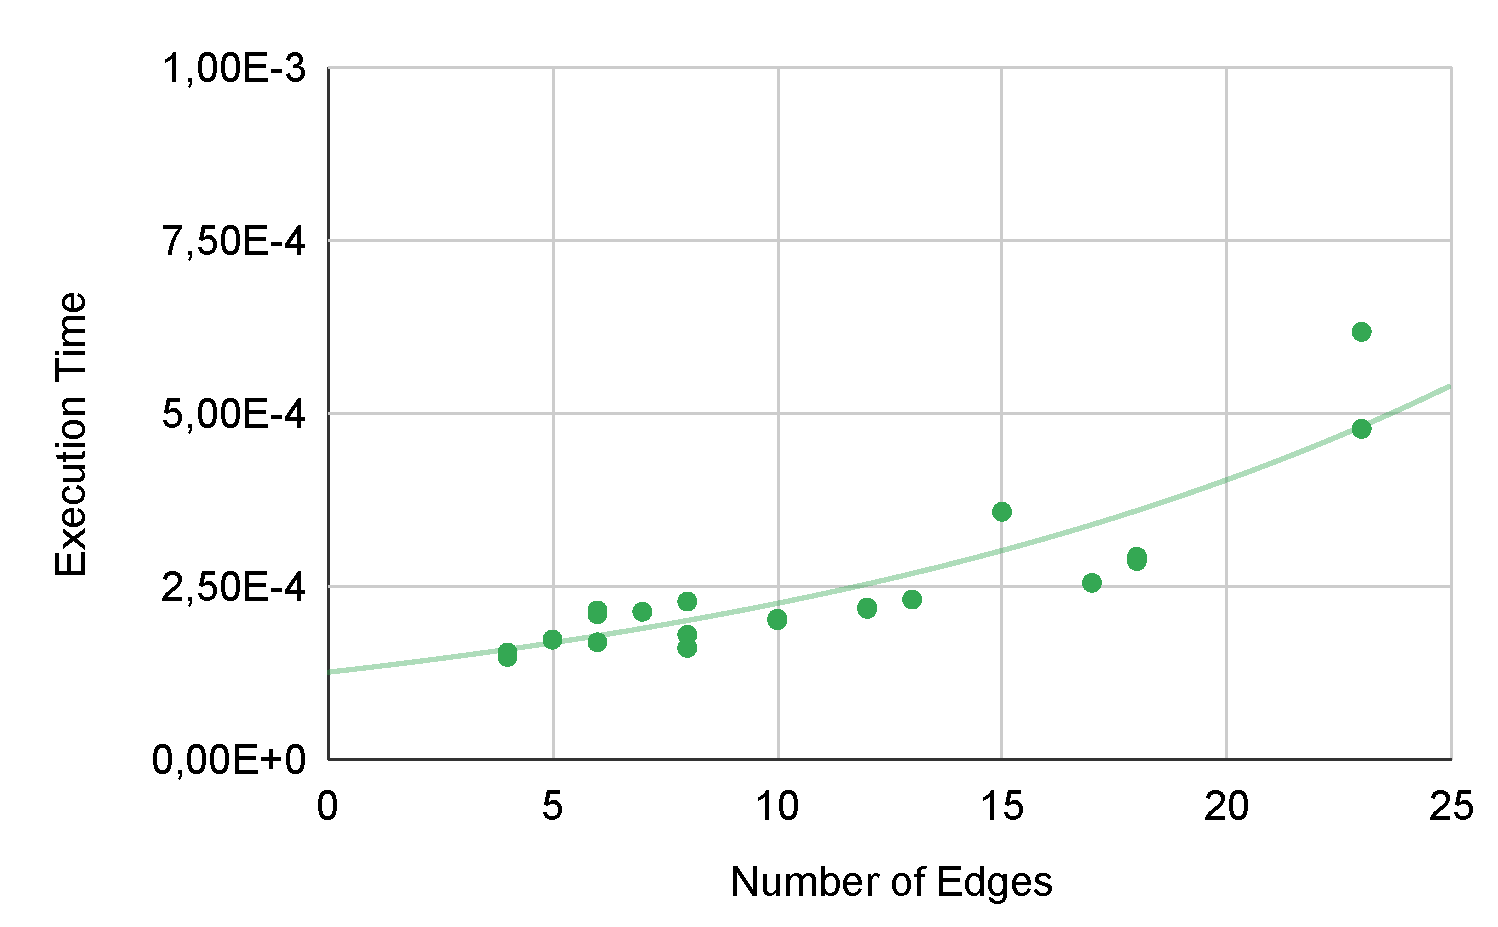
\includegraphics[width=0.9\linewidth]{figs/maxc-time.pdf}
    \caption{Correlation between number of edges and elapsed time for maximum connection greedy algorithm.}
    \label{fig:maxc-time}
\end{figure}


\begin{figure}[!ht]
    \centering
    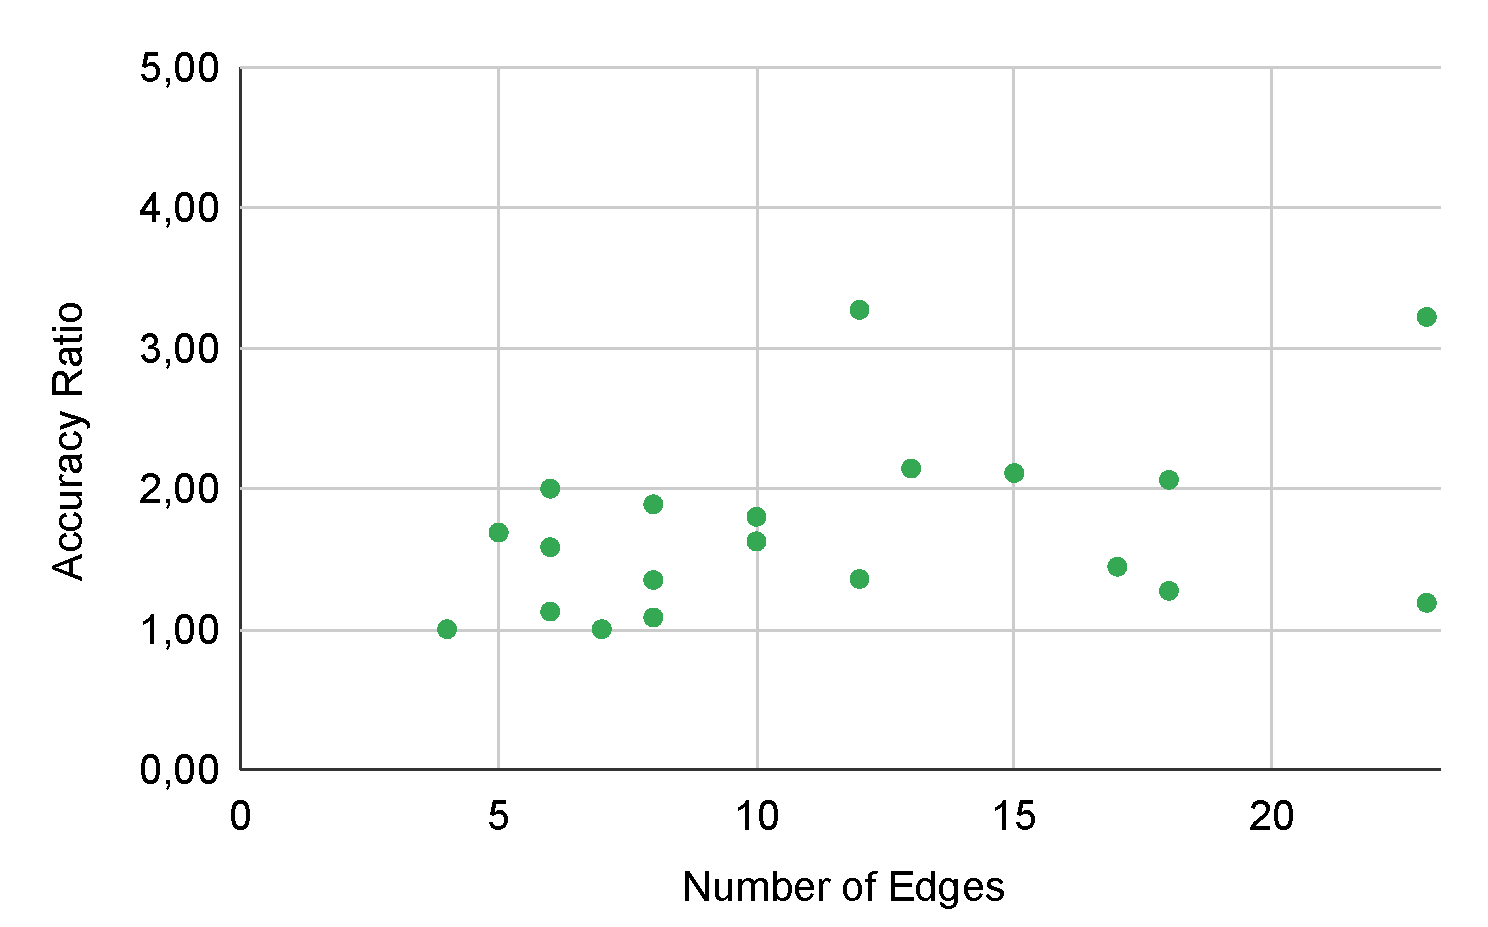
\includegraphics[width=0.9\linewidth]{figs/maxc-ratio.pdf}
    \caption{Correlation between number of edges and accuracy ratio for maximum connection greedy algorithm.}
    \label{fig:maxc-ratio}
\end{figure}

For the Chaurasia-Singh greedy heuristics, the results obtained are presented in \autoref{tab:chaurasia-table}, \autoref{fig:chaurasia-sol}, \autoref{fig:chaurasia-time}, and \autoref{fig:chaurasia-ratio}. 
The columns for \autoref{tab:chaurasia-table} are equal to the ones in \autoref{tab:minw-table}.
The data shows that the number of solutions tested grows with the number of edges, similar to both previous heuristics.
The elapsed time increases with the number of edges, very similarly to both previous heuristics.
The accuracy ratio for this algorithm is smaller then the two previous ones.


\begin{table}[ht!]
\caption{Results from Chaurasia-Singh greedy algorithm}
\label{tab:chaurasia-table}
\resizebox{0.5\textwidth}{!}{%
\begin{tabular}{ccccccc}
\multirow{3}{*}{V} & \multirow{3}{*}{p} & \multirow{3}{*}{E} & \multirow{3}{*}{\begin{tabular}{c} Execution \\ Time (s) \end{tabular}} & \multirow{3}{*}{\begin{tabular}{c}\# of\\ Solutions\\Tested\end{tabular}} & \multirow{3}{*}{\begin{tabular}{c} Accuracy \\ Ratio \end{tabular}}\\ 
& & & & & & \\
& & & & & & \\
\hline
4 & 0.125 & 4 & 1,61E-04 & 1 & 1,80 \\
4 & 0.25 & 6 & 2,28E-04 & 2 & 1,00 \\
4 & 0.5 & 6 & 2,04E-04 & 2 & 1,00 \\
4 & 0.75 & 6 & 2,13E-04 & 2 & 1,00 \\
5 & 0.125 & 4 & 1,51E-04 & 1 & 1,00 \\
5 & 0.25 & 6 & 2,38E-04 & 2 & 1,00 \\
5 & 0.5 & 7 & 2,28E-04 & 2 & 1,00 \\
5 & 0.75 & 8 & 2,48E-04 & 2 & 1,00 \\
6 & 0.125 & 5 & 2,19E-04 & 2 & 1,50 \\
6 & 0.25 & 8 & 2,14E-04 & 3 & 1,61 \\
6 & 0.5 & 12 & 2,31E-04 & 3 & 1,00 \\
6 & 0.75 & 13 & 2,38E-04 & 3 & 1,00 \\
7 & 0.125 & 6 & 1,87E-04 & 3 & 1,00 \\
7 & 0.25 & 10 & 2,10E-04 & 3 & 1,60 \\
7 & 0.5 & 15 & 3,74E-04 & 3 & 1,56 \\
7 & 0.75 & 18 & 3,15E-04 & 3 & 1,27 \\
8 & 0.125 & 8 & 1,90E-04 & 3 & 1,00 \\
8 & 0.25 & 12 & 2,28E-04 & 3 & 1,00 \\
8 & 0.5 & 18 & 2,84E-04 & 3 & 1,31 \\
8 & 0.75 & 23 & 5,49E-04 & 4 & 1,75 \\
9 & 0.125 & 10 & 2,21E-04 & 3 & 2,13 \\
9 & 0.25 & 17 & 2,81E-04 & 3 & 2,56 \\
9 & 0.5 & 23 & 6,62E-04 & 3 & 4,44
\end{tabular}%
}
\end{table}

\begin{figure}[!ht]
    \centering
    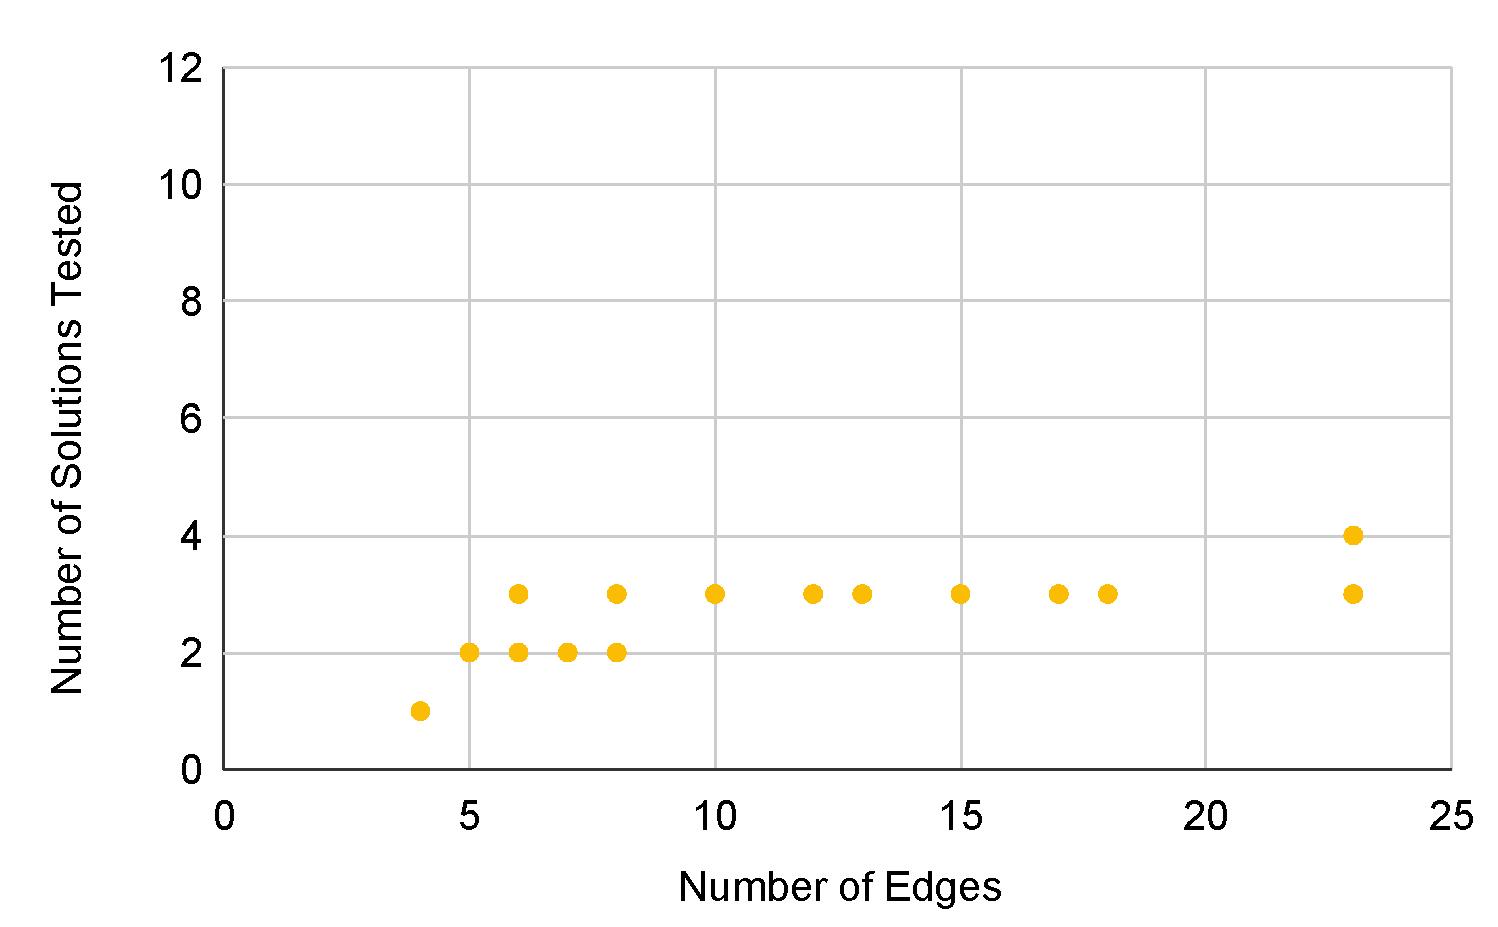
\includegraphics[width=0.9\linewidth]{figs/chaurasia-solutions.pdf}
    \caption{Correlation between number of edges and number of solutions tested for Chaurasia-Singh greedy algorithm.}
    \label{fig:chaurasia-sol}
\end{figure}


\begin{figure}[!ht]
    \centering
    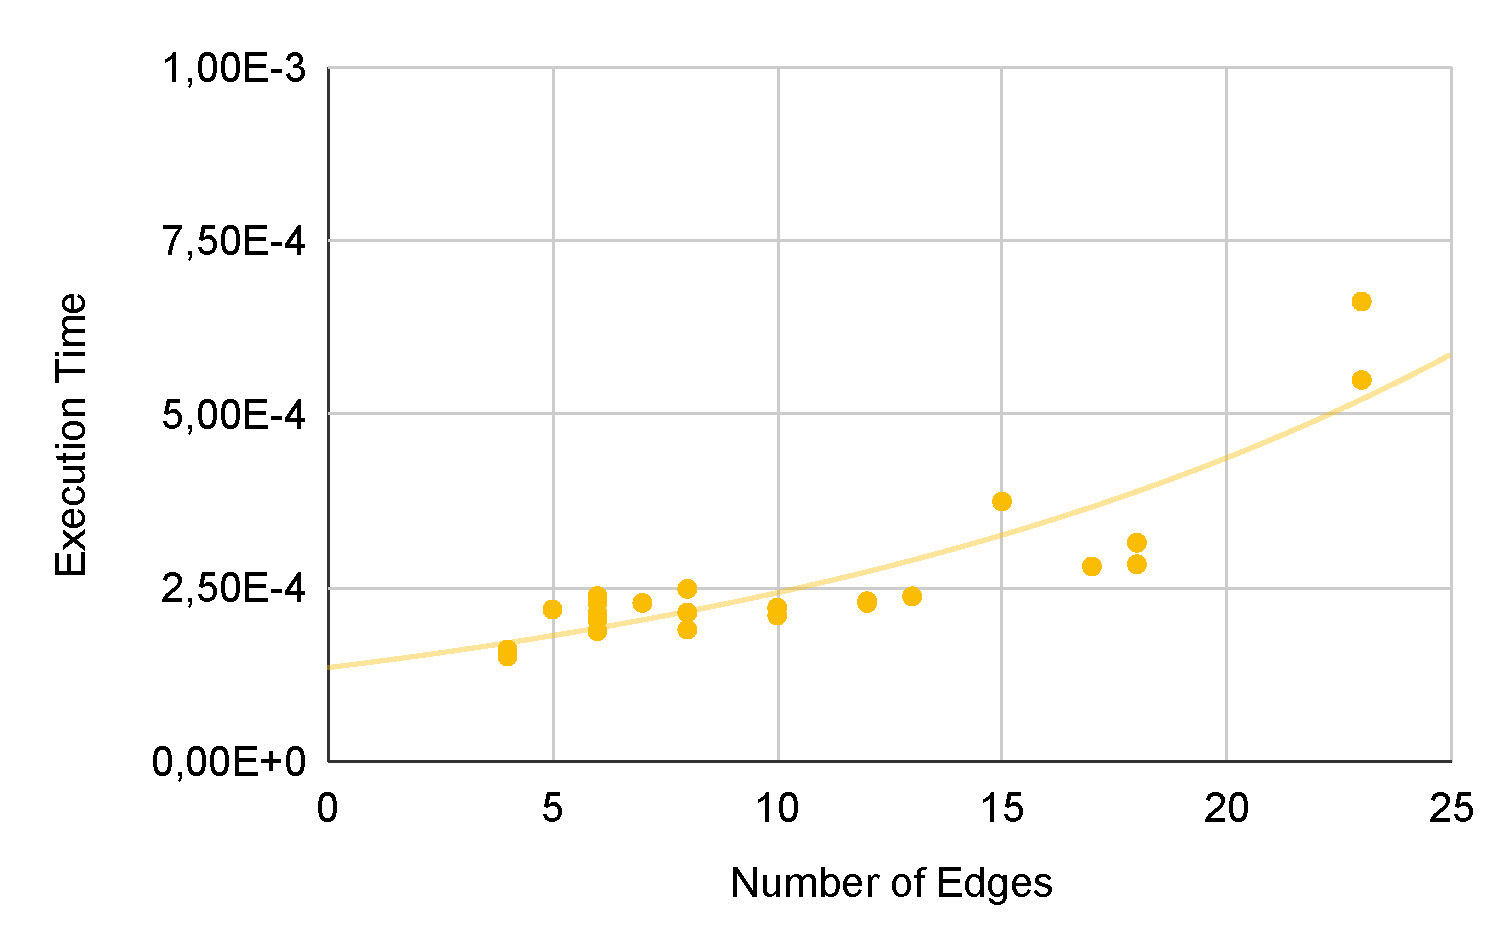
\includegraphics[width=0.9\linewidth]{figs/chaurasia-time.pdf}
    \caption{Correlation between number of edges and elapsed time for Chaurasia-Singh greedy algorithm.}
    \label{fig:chaurasia-time}
\end{figure}

\newpage

\begin{figure}[!ht]
    \centering
    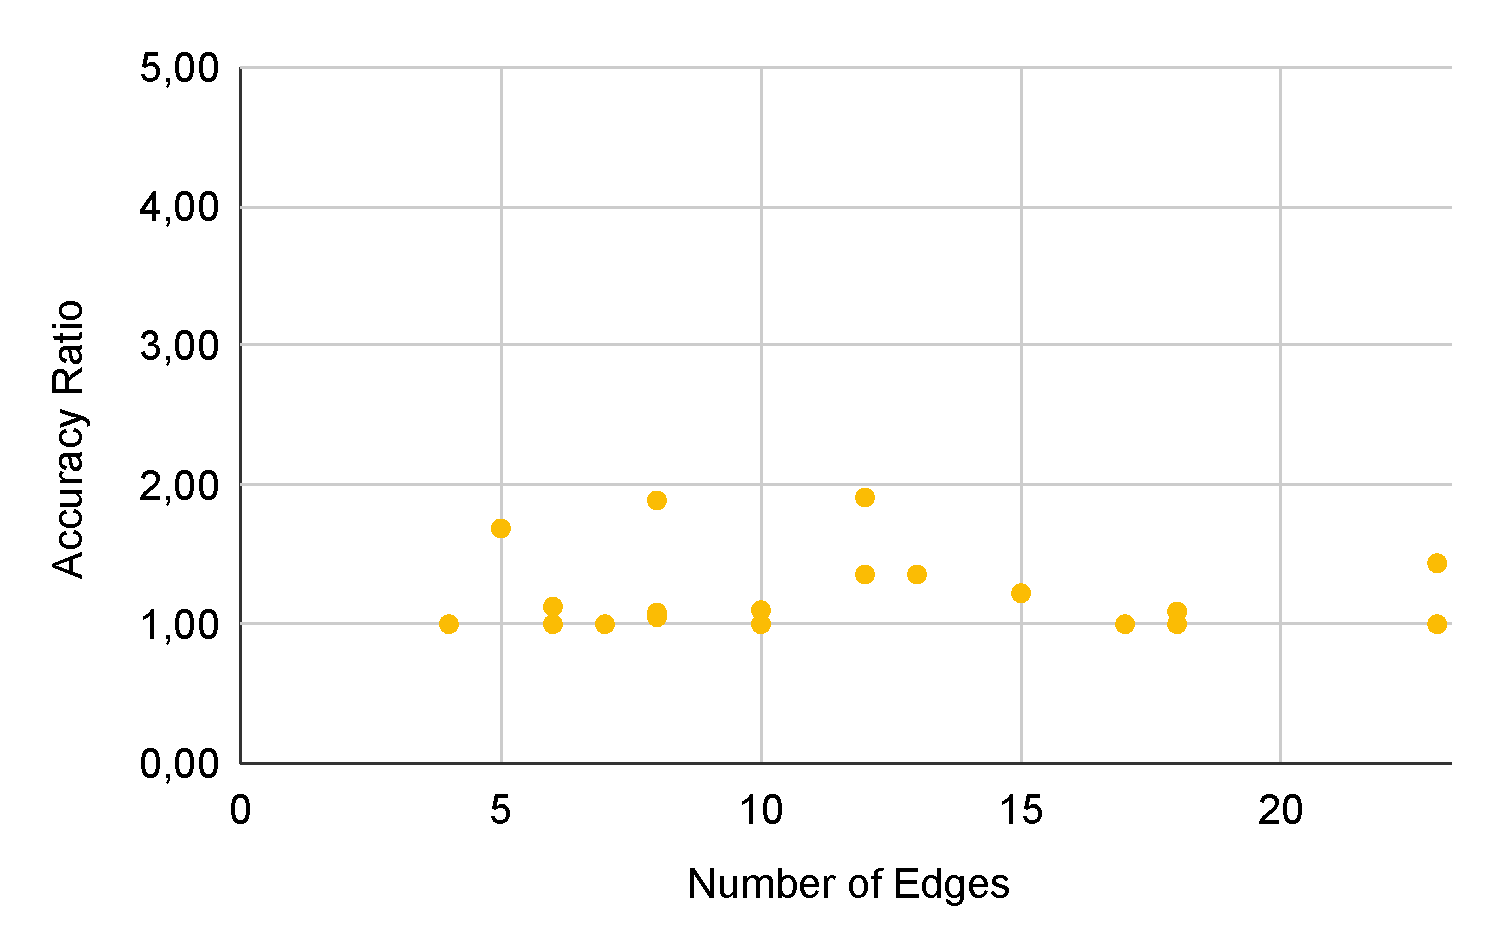
\includegraphics[width=0.9\linewidth]{figs/chaurasia-ratio.pdf}
    \caption{Correlation between number of edges and accuracy ratio for Chaurasia-Singh greedy algorithm.}
    \label{fig:chaurasia-ratio}
\end{figure}